\documentclass{article}
\usepackage{nips07submit_e,times}
\usepackage{amsmath}
\usepackage{subfig}
\usepackage{graphicx}

\title{Supplementary material for ``Model-based transcription factor
  target identification with limited data''}


\author{
Antti Honkela,
Neil D. Lawrence,
Charles Girardot, 
E. Hilary Gustafson,
Ya-Hsin Liu,\\
\bf Eileen E.M. Furlong, and
Magnus Rattray
}

% The \author macro works with any number of authors. There are two commands
% used to separate the names and addresses of multiple authors: \And and \AND.
%
% Using \And between authors leaves it to \LaTeX{} to determine where to break
% the lines. Using \AND forces a linebreak at that point. So, if \LaTeX{}
% puts 3 of 4 authors names on the first line, and the last on the second
% line, try using \AND instead of \And before the third author name.

\newcommand{\fix}{\marginpar{FIX}}
\newcommand{\new}{\marginpar{NEW}}
\newcommand{\erf}{\operatorname{erf}}

\begin{document}

\maketitle

%\begin{abstract}
%\end{abstract}

\section{Derivation of the Gaussian process model}

The linear system ODEs underlying our model is
\begin{align}
  \label{eq:translation_ode}
  \frac{df(t)}{dt} & = f(t) - \delta p(t) \\
  \label{eq:translation_ode}
  \frac{dm_j(t)}{dt} & = B_j + S_j p(t) - D_j m_j(t).
\end{align}
Assuming steady-state initial conditions $f(0) = 0$ and
$m_j(0) = B_j / D_j$, its solution is
\begin{align}
  \label{eq:protein_ode_sol}
  p(t) & = \exp(-\delta t) \int_0^t f(v) \exp(\delta v) \, dv \\
  \label{eq:mrna_ode_sol}
  m_j(t) & = \frac{B_j}{D_j} + S_j \exp(-D_j t) \int_0^t \exp(D_j
  u) \exp(-\delta u) \int_0^u f(v) \exp(\delta v) \, dv \, du.
\end{align}

Both of these are linear operators of $f(t)$.  Hence, placing a
Gaussian process prior on $f(t)$ implies a joint Gaussian process
model over all $(f(t), p(t), m_j(t))$~\cite{Rasmussen2006}.

This Gaussian process is completely characterised by its mean and
covariance functions.  Assuming $\mathrm{E}[f(t)] = 0$, the above
solutions (\ref{eq:protein_ode_sol})-(\ref{eq:mrna_ode_sol}) imply
$\mathrm{E}[p(t)] = 0$, $\mathrm{E}[m_j(t)] = B_j / D_j$.

What remains is to determine the covariance functions.  These can
be evaluated as expectations
\begin{equation}
  \label{eq:kernel_definition}
  k_{xy}(t,t') = \mathrm{E}[(x(t) - \mathrm{E}[x(t)])(y(t') - \mathrm{E}[y(t')])],
\end{equation}
where $x,y \in \{f, p, m_j\}$.  Assuming the squared exponential
covariance for $f(t)$,
\begin{equation}
  \label{eq:sqexp_kernel}
  k_{ff}(t, t') = a \exp\left( -\frac{(t-t')^2}{l^2} \right),
\end{equation}
all the required covariance functions can be derived in closed form
by repeated application of the identity
\begin{multline}
  \label{eq:gpsim_identity}
  \int_0^t \exp(D u) \erf(u/l + E)\,du =
  \frac{1}{D} \bigg[
  \exp(Dt) \erf(E + t/l) - \erf(E) \\
  + \exp\left(\left( \frac{Dl}{2}\right)^2 -E Dl \right)
  [ \erf(E - Dl/2) - \erf(E-Dl/2+t/l) ]
  \bigg].
\end{multline}

\subsection{Covariance function $k_{fp}$}

The covariance $k_{fp}$ is the same as the cross-covariance derived
in~\cite{Lawrence2007}:
\begin{align*}
  k_{fp}(t, t') &= \exp(-\delta t) \int_0^{t} \exp(\delta u) k_{ff}(u, t') du \\
   &= \frac{\sqrt{\pi}al}{2} \exp\left(\left(\frac{\delta l}{2}\right)^2 + \delta (t - t') \right)
   [\erf(\delta l / 2 + t/l) - \erf(\delta l / 2 + (t-t')/l)]
\end{align*}

\subsection{Covariance function $k_{fm_j}$}

\begin{multline}
  k_{f m_j}(t, t') = S_j \exp(-D_j t') \int_0^{t'}
  \exp((D_j - \delta) u) \int_0^u \exp(\delta v) k_{ff}(t, v)\, dv\, du \\
  = S_j \frac{\sqrt{\pi} al}{2(\delta - D_j)} \exp(-(D_j+\delta) t')) \\
  \bigg(
  \exp\left(\left(\frac{D_j l}{2}\right)^2 + D_j t + \delta t' \right)
  [\erf(D_j l / 2 + t/l) - \erf(D_j l / 2 + (t-t')/l)] \\
  -
  \exp\left(\left(\frac{\delta l}{2}\right)^2 + \delta t + D_j t'\right)
  [\erf(\delta l / 2 + t/l) - \erf(\delta l / 2 + (t-t')/l)]
  \bigg)
\end{multline}

\subsection{Covariance function $k_{pp}$}

Again following~\cite{Lawrence2007},
\begin{align*}
  k_{p p}(t, t') &= \exp(-\delta (t +t')) \int_0^t \exp(\delta u)
  \int_0^{t'} \exp(\delta u') k_{ff}(u, u') du' du \\
  &= \frac{\sqrt{\pi}al}{4 \delta}
  \exp\left(\left(\frac{\delta l}{2}\right)^2 -\delta (t + t')\right) [ h(t', t) +
  h(t, t')],
\end{align*}
where
\begin{multline}
  \label{eq:gpsim_h}
  h(t', t) = 
  \bigg\{ \exp[2 \delta t ] \bigg[
       \erf\left(\left(\frac{\delta l}{2}\right) + \frac{t}{l} \right) - 
       \erf\left(\left(\frac{\delta l}{2}\right) + \frac{t-t'}{l} \right) \bigg] \\
  + \bigg[
       \erf\left(\left(\frac{\delta l}{2}\right) - \frac{t'}{l} \right) -
       \erf\left(\left(\frac{\delta l}{2}\right) \right) \bigg] \bigg\}.
\end{multline}

\subsection{Covariance function $k_{pm_j}$}

\begin{multline}
  \frac{k_{p m_j}(t, t')}{S_j \exp(-\delta t - D_j t')} = 
  \int_0^{t'} \exp((D_j - \delta) u') \int_0^t \exp(\delta v) \int_0^{u'}
  \exp(\delta v') k_{yy}(v, v')\, dv'\, dv\, du' \\
  = 
  \frac{\sqrt{\pi}al}{4\delta}\exp\left(\left(\frac{\delta l}{2}\right)^2\right)
  \bigg(
  \frac{2 \delta}{\delta^2 - D_j^2}
  [\erf(\delta l / 2 - t/l) - \erf(\delta l / 2)]\\
  +
  \frac{\exp((D_j - \delta)t')}{\delta - D_j}
  [2\erf(\delta l / 2) - \erf(\delta l / 2 - t'/l) - \erf(\delta l / 2 - t/l)] \\
  +
  \frac{\exp((D_j + \delta)t')}{\delta + D_j}
  [\erf(\delta l / 2 + t'/l) - \erf(\delta l / 2 - (t-t')/l)]\\
  +
  \frac{\exp(2\delta t + (D_j - \delta)t')}{\delta - D_j}
  [\erf(\delta l / 2 + (t-t')/l) - \erf(\delta l / 2 + t/l)]
  \bigg) \\
  + \frac{\sqrt{\pi}l}{2(\delta^2 - D_j^2)}
  \exp\left(\left(\frac{D_j l}{2}\right)^2\right)
  \bigg(
  \erf(D_j l/2 - t'/l) - \erf(D_j l/2) \\
  + \exp((D_j + \delta) t) [\erf(D_j l/2 + t/l) - \erf(D_j l/2 + (t-t')/l)]
  \bigg)
\end{multline}

\subsection{Covariance function $k_{m_j m_k}$}

The final covariance between target genes is
\begin{multline}
  k_{m_j m_k}(t, t') = S_j S_k \exp(-D_j t - D_k t')
  \int_0^t \exp((D_j - \delta) u)
  \int_0^{t'} \exp((D_k - \delta) u') \\
  \int_0^u \exp(\delta v) \int_0^{u'} \exp(\delta v') k_{ff}(v, v') \, dv'\, dv\, du'\, du \\
  = \frac{\sqrt{\pi} a l S_j S_k}{2} \bigg(
  h_{jk}(t, t', \delta) + h_{kj}(t', t, \delta) 
  - h_{jk}(t, t', D_j) - h_{kj}(t', t, D_k)
  \bigg)
\end{multline}
where
\begin{multline}
  h_{jk}(t, t', D_x) = 
  \exp\left(\left(\frac{D_x l}{2}\right)^2\right)
  \frac{\exp(-D_x t - D_k t')}{(D_x + \delta) (D_j - \delta)}
  \bigg\{ 
   \\
   %\frac{(D_k + \delta)\exp((D_k-\delta) t') - 2\delta}{(D_k^2-\delta^2)}
  \left(\frac{\exp((D_k-\delta) t') - 1}{D_k-\delta} +
    \frac{1}{D_k + D_x} \right)
  [\erf(D_x l/2 - t/l) - \erf(D_x l/2)]
  \\
  + \frac{\exp((D_k+D_x)t')}{D_k+D_x}
  [\erf(D_x l/2 + t'/l)
  - \erf(D_x l/2 - (t-t')/l)]
  \bigg\} \\
\end{multline}

\section{Distance from predicted targets to closest TF binding sites}

Cumulative distributions of distances from predicted targets to the
closest TF binding site in the ChIP-chip data are presented in
Figs.~\ref{fig:dros_binding_site_distances_global} and
\ref{fig:dros_binding_site_distances_focused}.

\begin{figure}[p]
  \centering
  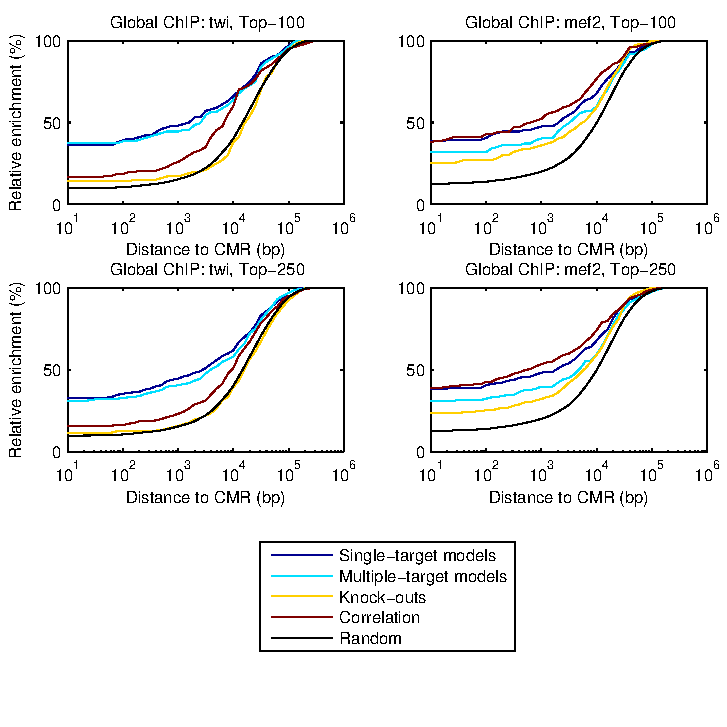
\includegraphics{dros_binding_site_distances_global}
  \caption{The fraction of predicted targets having a ChIP-chip
    binding site or CRM within $x$ base pairs as a function of $x$
    in the global ChIP-chip evaluation.
    \label{fig:dros_binding_site_distances_global}}
\end{figure}

\begin{figure}[p]
  \centering
  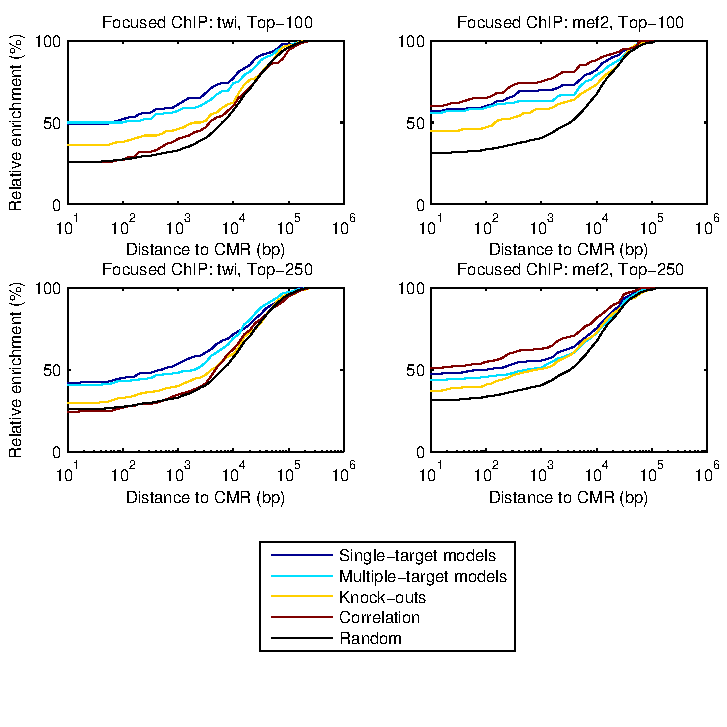
\includegraphics{dros_binding_site_distances_focused}
  \caption{The fraction of predicted targets having a ChIP-chip
    binding site or CRM within $x$ base pairs as a function of $x$
    in the focused ChIP-chip evaluation.
    \label{fig:dros_binding_site_distances_focused}}
\end{figure}

\section{Bootstrap sampling to estimate significance of differences of
  ranking methods}

The significance of the differences between different ranking methods
was estimated using bootstrap sampling.  We drew $100.000$ bootstrap
resamples of the data and repeated the ranking for each one of them.
We then recorded for each pair of methods, how often one of them was
better than the other.  It should be noted that these values are not
$p$-values nor directly transferable to be such.

The results of the sampling are presented below in
Tables~\ref{tab:bootstrap1}--\ref{tab:bootstrap6}.  The methods
studied are: ST = proposed single-target method, MT = proposed
multiple-target method, CO = ranking by correlation, KO = ranking by
$q$-value in knock-outs.  For each pair of methods, the marks in the
tables show how often the method on the corresponding row dominated
the one on the corresponding column.  The marks are interpreted as
follows: '.': $> 70 \%$ dominance, '+': $> 80 \%$ dominance,
'*': $> 90 \%$ dominance, '**': $> 95 \%$ dominance, '***': $> 99 \%$
dominance, '-': comparison not applicable.

\begin{table}[p]
  \centering
\subfloat[][Top 20]{
\begin{tabular}{lcccc}
    & ST  & MT  & CO  & KO \\
ST &     &     & .   & ***\\ 
MT &     &     & +   & ***\\ 
CO &     &     &     & ***\\ 
KO &     &     &     &    \\ 
\end{tabular}}
\subfloat[][Top 100]{
\begin{tabular}{lcccc}
    & ST  & MT  & CO  & KO \\
ST &     & .   & **  & ***\\ 
MT &     &     & *   & ***\\ 
CO &     &     &     & ***\\ 
KO &     &     &     &    \\ 
\end{tabular}}
\subfloat[][Top 250]{
\begin{tabular}{lcccc}
    & ST  & MT  & CO  & KO \\
ST &     & *   & *** & ***\\ 
MT &     &     & *** & ***\\ 
CO &     &     &     & ***\\ 
KO &     &     &     &    \\ 
\end{tabular}}
  \caption{Bootstrap results: Twist global ChIP-chip}
  \label{tab:bootstrap1}
\end{table}

\begin{table}[p]
  \centering
\subfloat[][Top 20]{
\begin{tabular}{lcccc}
    & ST  & MT  & CO  & KO \\
ST &     &     &     & -  \\ 
MT &     &     &     & -  \\ 
CO &     &     &     & -  \\ 
KO & -   & -   & -   & -  \\ 
\end{tabular}}
\subfloat[][Top 100]{
\begin{tabular}{lcccc}
    & ST  & MT  & CO  & KO \\
ST &     &     & **  & -  \\ 
MT &     &     & **  & -  \\ 
CO &     &     &     & -  \\ 
KO & -   & -   & -   & -  \\ 
\end{tabular}}
\subfloat[][Top 250]{
\begin{tabular}{lcccc}
    & ST  & MT  & CO  & KO \\
ST &     &     & *** & -  \\ 
MT &     &     & *** & -  \\ 
CO &     &     &     & -  \\ 
KO & -   & -   & -   & -  \\ 
\end{tabular}}
  \caption{Bootstrap results: Twist global knock-outs}
  \label{tab:bootstrap2}
\end{table}

\begin{table}[p]
  \centering
\subfloat[][Top 20]{
\begin{tabular}{lcccc}
    & ST  & MT  & CO  & KO \\
ST &     &     & **  & +  \\ 
MT &     &     & *   & +  \\ 
CO &     &     &     &    \\ 
KO &     &     &     &    \\ 
\end{tabular}}
\subfloat[][Top 100]{
\begin{tabular}{lcccc}
    & ST  & MT  & CO  & KO \\
ST &     & +   & *** & ***\\ 
MT &     &     & **  & ** \\ 
CO &     &     &     &    \\ 
KO &     &     &     &    \\ 
\end{tabular}}
\subfloat[][Top 250]{
\begin{tabular}{lcccc}
    & ST  & MT  & CO  & KO \\
ST &     & **  & *** & ***\\ 
MT &     &     & **  & ***\\ 
CO &     &     &     &    \\ 
KO &     &     &     &    \\ 
\end{tabular}}
  \caption{Bootstrap results: Twist focused ChIP-chip}
  \label{tab:bootstrap3}
\end{table}

\begin{table}[p]
  \centering
\subfloat[][Top 20]{
\begin{tabular}{lcccc}
    & ST  & MT  & CO  & KO \\
ST &     & +   & .   &    \\ 
MT &     &     &     &    \\ 
CO &     &     &     &    \\ 
KO &     & .   & .   &    \\ 
\end{tabular}}
\subfloat[][Top 100]{
\begin{tabular}{lcccc}
    & ST  & MT  & CO  & KO \\
ST &     & +   &     & +  \\ 
MT &     &     &     & .  \\ 
CO & +   & *   &     & ** \\ 
KO &     &     &     &    \\ 
\end{tabular}}
\subfloat[][Top 250]{
\begin{tabular}{lcccc}
    & ST  & MT  & CO  & KO \\
ST &     & *** &     & ** \\ 
MT &     &     &     &    \\ 
CO & *   & *** &     & ***\\ 
KO &     &     &     &    \\ 
\end{tabular}}
  \caption{Bootstrap results: Mef2 global ChIP-chip}
  \label{tab:bootstrap4}
\end{table}

\begin{table}[p]
  \centering
\subfloat[][Top 20]{
\begin{tabular}{lcccc}
    & ST  & MT  & CO  & KO \\
ST &     &     & .   & -  \\ 
MT &     &     & .   & -  \\ 
CO &     &     &     & -  \\ 
KO & -   & -   & -   & -  \\ 
\end{tabular}}
\subfloat[][Top 100]{
\begin{tabular}{lcccc}
    & ST  & MT  & CO  & KO \\
ST &     & +   & .   & -  \\ 
MT &     &     &     & -  \\ 
CO &     &     &     & -  \\ 
KO & -   & -   & -   & -  \\ 
\end{tabular}}
\subfloat[][Top 250]{
\begin{tabular}{lcccc}
    & ST  & MT  & CO  & KO \\
ST &     & .   & +   & -  \\ 
MT &     &     &     & -  \\ 
CO &     &     &     & -  \\ 
KO & -   & -   & -   & -  \\ 
\end{tabular}}
  \caption{Bootstrap results: Mef2 global knock-outs}
  \label{tab:bootstrap5}
\end{table}

\begin{table}[p]
  \centering
\subfloat[][Top 20]{
\begin{tabular}{lcccc}
    & ST  & MT  & CO  & KO \\
ST &     &     & +   & .  \\ 
MT &     &     & +   & +  \\ 
CO &     &     &     &    \\ 
KO &     &     &     &    \\ 
\end{tabular}}
\subfloat[][Top 100]{
\begin{tabular}{lcccc}
    & ST  & MT  & CO  & KO \\
ST &     & +   &     & +  \\ 
MT &     &     &     & .  \\ 
CO & *   & **  &     & ** \\ 
KO &     &     &     &    \\ 
\end{tabular}}
\subfloat[][Top 250]{
\begin{tabular}{lcccc}
    & ST  & MT  & CO  & KO \\
ST &     & **  &     & *  \\ 
MT &     &     &     &    \\ 
CO & *** & *** &     & ***\\ 
KO &     &     &     &    \\ 
\end{tabular}}
  \caption{Bootstrap results: Mef2 focused ChIP-chip}
  \label{tab:bootstrap6}
\end{table}

\bibliographystyle{pnas}
\bibliography{disim}

\end{document}
